%----------------------------------------------------------------------------------
% Exemplo do uso da classe pucrs-ppgcc.cls. Veja o arquivo .cls
% para mais detalhes e instruções.
%----------------------------------------------------------------------------------

% Seleção de idioma da monografia. Por enquanto as únicas opções
% suportadas são 'portuguese' e 'english'
% Para impressão em frente e verso, use a opção 'twoside'. Da
% mesma forma, use 'oneside' para impressão em um lado apenas.
\documentclass[portuguese,twoside]{pucrs-ppgcc}
%\documentclass[english,twoside]{pucrs-ppgcc}

%----------------------------------------------------------------
% Coloque seus pacotes abaixo.
%
% Obs.: muitos pacotes de uso comum do LaTeX, como amsmath,
% geometry e url já são automaticamente incluídos pela classe
% (veja o arquivo .cls). Isso torna obrigatória a presença destes
% no sistema para o uso desta classe, mas ao mesmo tempo o uso se
% torna mais simples.  Recomendo a instalação da versão mais
% recente da distribuição TeXLive (para Windows e UNIXes):
% www.tug.org/texlive/
%
% Pacotes e opções já incluídas automaticamente:
%
% \RequirePackage[T1]{fontenc}[2005/09/27]
% \RequirePackage[utf8x]{inputenc}[2008/03/30]
% \RequirePackage[english,brazil]{babel}[2008/07/06]
% \RequirePackage[a4paper]{geometry}[2010/09/12]
% \RequirePackage{textcomp}[2005/09/27]
% \RequirePackage{lmodern}[2009/10/30]
% \RequirePackage{indentfirst}[1995/11/23]
% \RequirePackage{setspace}[2000/12/01]
% \RequirePackage{textcase}[2004/10/07]
% \RequirePackage{float}[2001/11/08]
% \RequirePackage{amsmath}[2000/07/18]
% \RequirePackage{amssymb}[2009/06/22]
% \RequirePackage{amsfonts}[2009/06/22]
% \RequirePackage{url}
% \RequirePackage[table]{xcolor}[2007/01/21]
%----------------------------------------------------------------
% Para inserção de figuras.
\usepackage{graphicx}
% Utilize a opção 'pdftex' se você estiver usando o pdflatex (que
% permite figuras em formatos como .jpg ou .png)
%\usepackage[pdftex]{graphicx}

% Para tabelas com elementos ocupando mais de uma linha
\usepackage{multirow}
% Para frações na mesma linha (ex. ⅓).
\usepackage{nicefrac}
% Para inserir figuras lado a lado.
% \usepackage{subfigure}
% Para formatar algoritmos.
% A opção [algo2e] é necessária para evitar conflitos
% com as definições da classe.
%\usepackage[algo2e]{algorithm2e}
\usepackage{algorithmic}
% Um float do tipo algoritmo. No momento
% este pacote é incompatível com a classe.
%\usepackage{algorithm}
\usepackage{booktabs}

\author{Bruno Rubin dos Santos Matheus Bonifácio Morais}
\title{OLAP Docking - Uma solução OLAP para análise de experimentos de docagem molecular: aplicação com a enzima I\MakeLowercase{nh}A.}
      {OLAP Docking - An OLAP solution to analyze molecular docking experiments: applied to I\MakeLowercase{nh}A enzyme.}

\tipotrabalho{\monografia}  % Monografias em geral (e de "bônus": TCCs)
\grau{\bacharel} 

\orientador{Duncan Dubugras Alcoba Ruiz}

\begin{document}

%----------------------------------------------------------------
% Depois da capa vem a dedicatória e a epígrafe.
%----------------------------------------------------------------
%\dedicatoria{Dedico este trabalho a meus pais.}

%\epigrafe{The art of simplicity is a puzzle of complexity.}
%         {Douglas Horton}

%----------------------------------------------------------------
% Também dá para fazer as duas na mesma página:
%----------------------------------------------------------------
%\dedigrafe{Dedico este trabalho a meus pais.}
%          {The art of simplicity is a puzzle of complexity.}
%          {Douglas Horton}

%----------------------------------------------------------------
% A seguir, a página de agradecimentos (OPCIONAL):
%----------------------------------------------------------------
%\begin{agradecimentos}
%À lorem ipsum, dolor sit amet consetetur sadipscing elitr sed diam
%nonumy eirmod tempor. invidunt ut labore et dolore magna aliquyam
%
%À erad sed, diam voluptua at vero, eos et accusam et justo duo
%dolores et ea rebum stet clita.
%
%À kasd gubergren, no sea. takimata sanctus est lorem ipsum dolor sit
%amet lorem ipsum dolor sit amet. consetetur sadipscing elitr sed
%
%À diam nonumy, eirmod tempor, invidunt ut labore et dolore magna
%aliquyam erat sed diam voluptua at.
%\end{agradecimentos}

%----------------------------------------------------------------
% Resumo, com as palavras-chave passadas por parâmetro
% (OBRIGATÓRIO, ao menos para teses e dissertações)
%----------------------------------------------------------------
\begin{resumo}{OLAP, InhA, Docagem Molecular}

O processo de desenvolvimento de novos fármacos é uma atividade fundamental para a indústria farmacêutica, na qual é utilizado não somente para o desenvolvimento de novos compostos para atender uma determinada necessidade, mas também tem como objetivo evoluir os compostos já existentes em busca de um resultado aprimorado e mais eficaz. A área de bioinformática tem como um de seus objetivos, através do uso de recursos e técnicas computacionais, acelerar e aprimorar o processo de desenvolvimento de medicamentos.
Esse processo consiste na análise das interações entre pequenas moléculas e receptores, e o processo de docagem molecular, é o responsável por simular e avaliar de forma qualitativa as interações estabelecidas.  O principal desafio para a realização destes experimentos é quando a flexibilidade do receptor é considerada. Para este caso, é utilizado um conjunto de conformações (snapshots) gerados apartir de simulações por dinâmica molecular.
A análise dos dados resultantes de docagem é feita de forma manual pelo especialista de domíno através do uso de um protocolo para avaliação. Os dados gerados pelas simulações crescem de acordo com o conjunto de snapshots que é utilizado, dificultando a análise e visualização de todos os resultados. 

\end{resumo}

%----------------------------------------------------------------
% Abstract, com as palavras-chave passadas por parâmetro
% (OBRIGATÓRIO, ao menos para teses e dissertações)
%----------------------------------------------------------------
\begin{abstract}{lorem, ipsum, dolor, sit, amet}
Your abstract in English here. lorem ipsum dolor sit amet
consetetur sadipscing elitr sed diam nonumy eirmod tempor invidunt
ut labore et dolore magna aliquyam erat sed diam voluptua at vero
eos et accusam et justo duo dolores et ea rebum stet clita kasd
gubergren no sea takimata sanctus est lorem ipsum dolor sit amet
lorem ipsum dolor sit amet consetetur sadipscing elitr sed diam
nonumy eirmod tempor invidunt ut labore et dolore magna aliquyam
erat sed diam voluptua at
\end{abstract}

%----------------------------------------------------------------
% Listas e sumário, nessa ordem. Somente o sumário é obrigatório,
% portanto, comente as outras listas, caso sejam desnecessárias.
%----------------------------------------------------------------
\listoffigures       % Lista de figuras      (OPCIONAL)
\listoftables        % Lista de tabelas      (OPCIONAL)
%\listofalgorithms    % Lista de algoritmos   (OPCIONAL)
\listofacronyms      % Lista de siglas       (OPCIONAL)
%\listofabbreviations % Lista de abreviaturas (OPCIONAL)
%\listofsymbols       % Lista de símbolos     (OPCIONAL)
\tableofcontents     % Sumário               (OBRIGATÓRIO)


\sigla{3D}		{Tridimensional}
\sigla{BD}		{Banco de Dados}
\sigla{CADD}	{\emph{Computer-aided drug design} ou desenvolvimento de fármacos auxiliado por computador}
\sigla{DM}		{Dinâmica Molecular}
\sigla{ETH}		{Etionamida}
\sigla{FEB}		{\emph{Free Energy of Binding} ou Energia Livre de Ligração}
\sigla{InhA}	{Enzima 2-trans-Enoil ACP(CoA) Reductase de Mycobacterium tuberculosis }
\sigla{LABIO}	{Laboratório de Bioinformática, Modelagem e Simulação de Biossistemas}
\sigla{NADH}	{Resíduo Nicotinamida Adenina Dinucleotídeo}
\sigla{PDB}		{\emph{Protein Data Bank} ou Banco de Dados de Proteínas}
\sigla{RDD}		{\emph{Rational Drug Design} ou Planejamento Racional de Fármacos}
\sigla{RMSD}	{\emph{Root Mean Square Deviation} ou Desvio Médio Quadrático}
\sigla{TCL} 	{Triclosano}
\sigla{CSV} 	{Comma-separated values}
\sigla{OLAP} 	{Online Analytical Processing}
\sigla{SQL} 	{Structured Query Language}



%----------------------------------------------------------------
% Aqui começa o desenvolvimento do trabalho. Para uma melhor
% organização do documento, separe-o em arquivos,
% um para cada capítulo. Para isso, utilize o comando \include,
% como mostrado abaixo.
%----------------------------------------------------------------
\chapter{Introdução}
\section{Caracterização do problema}
O processo de desenvolvimento de novos fármacos é uma atividade fundamental para a indústria farmacêutica, na qual é utilizado não somente para o desenvolvimento de novos compostos para atender uma determinada necessidade, mas também tem como objetivo evoluir os compostos já existentes em busca de um resultado aprimorado e mais eficaz. 

Este processo possui uma alta complexidade e exige, em média, 14 anos desde a identificação até a liberação pelo órgão regulador. As etapas envolvidas neste processo vão desde a identificação de um possivel candidato à fármaco, seguido por uma pesquisa de otimização, testes \emph{in-silico} e \emph{in-vitro}, análises toxicológicas até os ensaios clínicos. Estima-se que os custos de desenvolvimento de um novo fármaco seja aproximadamente de 1,2 bilhões de dólares \cite{kun92}. 

A área de bioinformática tem como um de seus objetivos, através do uso de recursos e técnicas computacionais, auxiliar o processo de descobrimento de novos fármacos. A partir de algoritmos computacionais é possível realizar simulações para identificar possíveis candidatos a novos fármacos e, posteriormente, submetê-los a testes mais específicos. Estes testes e simulações executados com auxílio computacional são denominados \emph{in-silico}.

O fator de desenvolvimento constante de novos \emph{softwares} e \emph{hardwares} contribui para que experimentos deste tipo sejam executados de forma cada vez mais rápida e com um maior nível de precisão. Esta metodologia passou a ser utilizada exaustivamente pelas indústrias farmacêuticas por se tratar de um método que exige um menor custo financeiro, se comparado com os tradicionais testes em laboratório \cite{art08}. 

O LABIO (Laboratório de Bioinformática, Modelagem e Simulação de Biossistemas) da Faculdade de Informática da Pontifícia Universidade 
Católica do Rio Grande do Sul (PUCRS) realiza pesquisas e estudos \emph{in-silico} de interações entre a enzima InhA (\emph{Mycobacterium 
tuberculosis}) e seus resíduos, que possam apresentar ligações receptor-ligante estáveis através de simulações de docagem molecular.

Dentro do processo de desenvolvimento de fármacos, a docagem molecular pode ser considerada como o principal método para avaliar a eficácia das combinações químicas entre as conformações. A docagem molecular é um método a qual prediz a orientação preferencial de encaixe de uma molécula à outra, com o objetivo de formar um complexo receptor-ligante estável. Este método pode ser simulado computacionalmente através dos algoritmos de docagem. 

A docagem basicamente envolve duas moléculas, uma chamada de receptor, que normalmente é uma proteína, e um ligante que á a molécula complementar que se conecta ao receptor. A avaliação do resultado da ligação estabelecida entre as duas moleculas se dá pelo cálculo de duas propriedades, uma é chamada de energia livre de ligação (Free energy of binding) e a outra é chamada de RMSD (Root mean square deviation). Analisar esta interação entre o receptor e o ligante não é uma tarefa simples visto que estes são influenciados por uma série de fatores ambientais. Os algoritmos de docagem precisam levar em consideração todas as formas de ligação entre o ligante e o receptor, o que inclui a exploração de todos os graus de liberdade translacionais e rotacionais do ligante, além dos graus de liberdade conformacionais do receptor.

O principal desafio da realização de testes \emph{in-silico} é quando a flexibilidade da molécula receptora passa a ser considerada. Devido ao tamanho da molécula e sua complexidade, as simulações com receptores flexíveis requerem um grande esforço computacional para realização dos cálculos necessários \cite{art08}.
Existem diversas abordagens para contornar este problema, e uma delas é a utilização de conjuntos de conformações gerados em simulações por Dinâmica Molecular (DM). Esta técnica consiste em gerar um conjunto de conformações de uma proteina em um intervalo de tempo, tendo como objetivo principal o estudo do comportamento dinâmico e também da geometria de uma proteína. Cada conformação em um instante de tempo específico é denominada \emph{snapshot} e possui propriedades que podem ser calculadas. Com isso, é executado uma simulação de docagem molecular para cada \emph{snapshot} do conjunto gerado por DM.

Todavia, apesar das metologias que geram um conjunto de conformações representativas do comportamento dinâmico de um receptor, a análise dos dados resultantes das simulações de docagem molecular ainda se faz de forma manual pelo especialista de domíno. A análise das interações ligante-receptor acaba se tornando humanamente inviável de ser feita para todos os resultados da docagem, pois o especialista possui um protocolo utilizado para avaliar de forma manual estes resultados, através dos valores de FEB (Free Energy of Binding) e RMSD (Root-mean-square Deviation), e também a geometria resultante.

Estima-se que a análise dos dados resultantes, seguindo o protocolo utilizado pelo especialista, necessitaria de aproximadamente 516 horas (mais de 21 dias) para ser concluída para todos os resultados de apenas uma molécula ligante, se fosse utilizado uma dinâmica molecular de 3.100 conformações (levando em consideração o tempo médio de análise de 10 minutos por conformação). Este número se torna ainda mais expressivo para uma simulação utilizando uma dinâmica molecular de 20.000 conformações, atualmente em uso no LABIO.


\section{Motivação}

Dados da Organização Mundial da Saúde confirmam que a Tuberculose (TB) é a segunda doença infecciosa que mais causa mortes em todo o mundo, perdendo apenas para o HIV/AIDS. No ano de 2012, 8.6 milhões de pessoas foram diagnosticadas com Tuberculose e 1.3 milhões morreram por estarem infectadas. A Tuberculose, causada pela bactéria \emph{Mycobacterium tuberculosis}, embora seja curável, é uma preocupação de nível mundial.

Atualmente existem programas governamentais que se esforçam no controle e no combate à TB, que tem como objetivo principal evitar que a doença seja difundida entre a população. Para o tratamento da doença, existem três principais fármacos que são utilizados: isoniazida (INH), rifampicina (RMP) e pirazinamida (PZA). O tratamento realizado com estes fármacos tem duração, em média, de 6 meses. Se não houver colaboração do paciente e o tratamento for interrompido de forma precoce, pode gerar bactérias resistentes à estes compostos químicos, sendo mais difíceis de combater. Devido aos efeitos colaterais destes medicamentos, muitas vezes o tratamento não é concluído adaquadamente, criando bactérias mais resistentes.

O desenvolvimento de novos fármacos ou a melhoria de compostos químicos já existentes é um esforço necessário para controle e combate a Tuberculose. O processo de CADD, desenvolvimento de fármacos auxiliado por computador (do inglês \emph{Computer-aided drug design}), é utilizado em larga escala para testes \emph{in-silico}, com objetivo de identificar novos compostos que mostrem eficácia e minimizem os efeitos colaterais aos pacientes.

Além da motivação relacionada ao receptor InhA que está sendo utilizado neste trabalho, uma das principais motivações está em contribuir com a comunidade de bioinformática e com o LABIO da PUCRS na pesquisa e desenvolvimento de métodos para cura e controle desta doença, através do desenvolvimento de uma ferramenta que auxilie a análise dos dados resultantes de experimentos realizados. 

Poranto, a utilização da ferramenta desenvolvida neste trabalho permitirá ao especialista de domínio uma maior chance de identificar ligações estáveis em um menor período de tempo, sem que haja conhecimentos avançados de informática e sem necessitar de recursos computacionais de alta capacidade.

\section{Objetivos}
\subsection{Objetivo geral}
O objetivo deste trabalho é contribuir com a análise dos resultados de simulações de docagem molecular através do desenvolvimento de um modelo OLAP e de todo o processo de extração, transformação e carga de dados, de forma a organizar estes resultados sob uma estrutura de cubos, e possibilitar, ao especialista de domínio, a realização de uma análise multidimensional das informações ali presentes e a obtenção de informações relevante de uma maneira mais rápida e menos custosa.

\subsection{Objetivos específicos}
\begin{itemize}
	\item Desenvolver um conjunto de scripts para preparação de dados de simulações de docagem molecular para carga no modelo OLAP.
	\item Desenvolver um modelo OLAP baseado em um banco de dados utilizado para armazenamento de resultados de docagem molecular.
	\item Permitir aos especialistas de domínio o cruzamento das informações de uma simulação por agrupamento de conformações.
	\item Contribuir para que os resultados das simulações de docagem molecular possam ser analisados multidimensionalmente, facilitando a identificação de complexos receptor-ligantes estáveis.
\end{itemize}

\section{Organização do documento}

Este documento está organizado da seguinte maneira:

\begin{itemize} 
	\item O Capítulo 2 apresenta os conceitos fundamentais para entendimento do trabalho desenvolvido, como: planejamento racional de fármacos, dinâmica molecular e o processo de docagem molecular. Ainda neste capítulo são apresentados conceitos de modelos multidimensionais OLAP e processo de ETL.
	\item No Capítulo 3 são apresentadas breves descrições das ferramentas que foram empregadas para o desenvolvimento deste trabalho, como a linguagem Python e o Microsoft SQL Analysis Services respectivamente.
	\item O Capítulo 4 descreve os elementos envolvidos na modelagem deste trabalho, bem como a fonte de dados utilizada para extração das informações.
	\item No Capítulo 5 são apresentadas todas as etapas envolvidas no processo de desenvolvimento do trabalho, desde identificação de métricas utilizadas, desenvolvimento de scripts para processo de ETL, concepção e definição das dimensões do modelo multidimensional, até por fim apresentar a construção do modelo OLAP em si.
	\item O Capítulo 6 apresenta as questões de negócio que foram possíveis responder utilizando o modelo OLAP desenvolvido e também as possibilidades de consultas e análise multidimensional dos dados.
	\item No Capítulo 7 são apresentadas as conclusões deste trabalho e também sugere algumas possibilidades para trabalhos futuros.
	
\end{itemize} 
% ----------------------------------------------------------
% Referencial Teórico
% ----------------------------------------------------------
\chapter{Referencial Teórico}

\section{Planejamento Racional de Fármacos}
Devido aos avanços da biologia, atualmente o processo de descoberta e desenvolvimento de novos compostos químicos capazes de prevenir ou curar doenças passou a seguir um planejamento racional, com embasamento lógico e teórico \cite{rdd}. Esse processo é denominado “Planejamento Racional de Fármacos” (do inglês RDD - \emph{Rational Drug Design}) e, de acordo com Kuntz \cite{kun92}, ele se divide em quatro etapas e está reprensentados através do \emph{workflow} da Figura \ref{fig:rddworkflow} \cite{kar11}: 

\begin{figure}[h]
	\center
	\includegraphics[width=14cm]{images/rdd_workflow.png}
	\caption{\emph{Workflow} do processo de planejamento racional de fármacos assistido por computador \cite{kar11}}
	\label{fig:rddworkflow}
\end{figure}


\begin{enumerate}
  \item O primeiro passo é definir um receptor (normalmente uma proteína) \cite{dre00} e analisar computacionalmente sua estrutura 3D. A estrutura da proteína é determinada por cristalografia por difração de raios X ou ressonância magnética nuclear \cite{far99}, sendo as informações resultantes armazenadas em um banco de dados como o Protein Data Bank - PDB \cite{ber00}. Essa análise tem por objetivo localizar possíveis regiões de ligação onde um ligante pode estabelecer ligações (atividades 1 e 2 do \emph{workflow} da Figura \ref{fig:rddworkflow});
  
  \item Baseado nas prováveis regiões de ligação identificadas no passo anterior, é selecionado um conjunto de possíveis candidatos, chamados ligantes (usualmente pequenas moléculas que podem ser buscadas em Banco de Dados de compostos como o ZINC \cite{irw05}) que podem se ligar a essa região no receptor (atividade 3 \emph{workflow} da Figura \ref{fig:rddworkflow}). As diferentes conformações que determinado ligante pode assumir dentro do sítio de ligação de uma determinada proteína são simuladas por softwares de docking como AutoDock 3.05 \cite{mor98} (atividade 4 do \emph{workflow} da Figura \ref{fig:rddworkflow});
  
  \item Os ligantes que teoricamente obtiveram melhores resultados nas simulções são experimentalmente sintetizados e testados (atividade 5 do \emph{workflow} da Figura \ref{fig:rddworkflow});
  
  \item Baseado nos resultados experimentais, o medicamento é gerado (atividade 6 do \emph{workflow} da Figura \ref{fig:rddworkflow}) ou o processo retorna ao passo 1.
  
\end{enumerate}
  
  Estas quatro etapas descritas por Kuntz \cite{kun92} contemplam apenas as fases de pesquisa e desenvolvimento de um novo medicamento. 
Somente após um longo período de pesquisas e testes \emph{in-vitro} e \emph{in-vivo}, estabelecendo eficácia e segurança, o novo fármaco é submetido para registro no órgão regulador.

A Tabela \ref{tab:rddtempo} apresenta, de uma forma geral, as etapas que envolvem o processo de desenvolvimento de um novo fármaco e o tempo médio de cada uma delas \cite{kun92}.

% Please add the following required packages to your document preamble:
% \usepackage{booktabs}
\begin{table}[h]
	\caption{Passos e tempo para desenvolvimento de um novo fármaco \cite{kun92}}
	\label{tab:rddtempo}
	\centering
	\begin{tabular}{@{}lc@{}}
	\toprule
	\multicolumn{1}{c}{\textbf{Passo}}      & \textbf{Tempo (Anos)} \\ \midrule
	Descoberta e geração de um candidato    & 1 - 2                 \\
	Otimização do candidato                 & 1 - 2                 \\
	Ensaios in-vitro e in-vivo              & 1 - 2                 \\
	Testes toxicológicos                    & 1 - 3                 \\
	Testes de segurança em humanos          & 1                     \\
	Testes de eficiência em humanos         & 1 - 2                 \\ \midrule
	\textbf{Tempo total de desenvolvimento} & \textbf{6 - 12}       \\ \bottomrule
	\end{tabular}
\end{table}

O desenvolvimento de fármacos auxiliado por computador (do inglês CADD - \emph{Computer-aided drug design}) consiste na utilização de recursos, ferramentas e técnicas computacionais contribui de forma significativa para as etapas de desenvolvimento de um fármaco.  Diferentes estágios deste processo podem ser beneficiados pelo uso da computação, podendo ser aplicado na identificação da molécula-alvo, planejamento, análise e melhoramento de ligantes.


\section{Dinâmica Molecular}

O advento da utilização de recursos computacionais aplicado às áreas medicinais e biológicas têm proporcionado o avanço de técnicas e uso de ferramentas que contribuem de forma expressiva para o planejamento racional de fármacos.

A Dinâmica Molecular (DM) é uma técnica de simulação computacional, fundamentada nos princípios da Mecânica Clássica, que possibilita o estudo do comportamento dinâmico microscópico de um sistema molecular, em diferentes intervalos de tempo \cite{nam08}. 

A simulação por DM fornece informações dos átomos que constituem o sistema molecular, permitindo o cálculo de diversas propriedades (pressão, temperatura, volume, energia livre, etc) e análise do potencial de interação dos ligantes na estrutura e estabilidade das proteínas \cite{kar11}.

De acordo com Lesk \cite{art08}, as interações entre os átomos em uma molécula podem ser classificadas de duas maneiras:

\begin{quote}
	(a) Ligações químicas primárias - interações fortes entre átomos que estão localizados bem próximos no espaço. São consideradas interações fixas pois são consistentes em um grande número de conformações, não sendo desfeitas ou alteradas quando a conformação de uma proteína muda. 

	(b) Interações mais fracas que dependem da conformação, podem ser significativas em algumas conformações e não em outras - elas afetam conjuntos de átomos que são aproximados devido a diferentes padrões de enovelamento da cadeia.
\end{quote}

As proteínas são corpos flexíveis que não possuem uma conformação única e fixa. Elas apresentam conformações que variam em um intervalo de tempo. A Figura \ref{fig:dm} ilustra a flexibilidade da enzima receptora InhA, onde cada cor representa uma conformação em um determinado instante de tempo \cite{COH10}.

\begin{figure}[h]
	\center
	\includegraphics[scale=0.4]{images/dm_inha.png}
	\caption{Flexibilidade da enzima receptora InhA. Sobreposição de diferentes conformações da InhA, representadas em fitas, durante uma simulação de DM. A conformação inicial da simulação está representada pela cor verde. Outras duas conformações foram capturadas pela simulação de DM nos intervalos de 1,000 ps (cor azul) e 3,000 ps (cor magenta). O retângulo tracejado identifica a região com maior flexibilidade \cite{REN13}.}
	\label{fig:dm}
\end{figure}

A conformação de uma proteína pode ser especificada pela lista de átomos na estrutura, por suas coordenadas e pelo conjunto de ligações químicas entre eles. A avaliação de uma conformação é feita através do cálculo de conjuntos de potenciais de energia. Estes calculos são computacionalmente complexos e intensivos, mas com a evolução rápida da capacidade de processamento dos computadores esta técnica é beneficiada diretamente \cite{art08}.

A simulação por DM se mostra um método versátil e acessível, sendo considerada a melhor técnica para geração de um conjunto de conformações de um receptor \cite{kar11}. Devido à isso, os dados dos conjuntos de conformações dos receptores utilizados neste trabalho foram gerados utilizando a DM.


\section{Docagem Molecular}

A Docagem Molecular é considerada um dos principais processo do CADD, e é através dela que são produzidos os dados detalhados sobre a interação entre receptores e seus ligantes \cite{LEN96}. 

No processo de Docagem Molecular, algoritmos de docagem são executados para testar e analisar virtualmente a interação entre um ligante e um receptor. Estes algoritmos geram um grande número de interações, onde em todas elas, o ligante é testado em diferentes orientações e conformações dentro do sítio de ligação do receptor, de modo a formar um complexo estável. 
Usualmente o receptor é uma proteína ou uma molécula de ácido nucléico, e o ligante pode ser uma pequena molécula ou até mesmo outra proteína. A Figura \ref{fig:docking} \cite{ALE13} ilustra cada um destes elementos e apresenta como é feita a interação entre eles.

\begin{figure}[h]
	\center
	\includegraphics[width=17cm]{images/docking.png}
	\caption{Representação do processo de docagem molecular em três dimensões (3D) entre uma proteína como receptor e uma pequena molécula como ligante, na qual se estabelece uma interação entre eles no sítio de ligação do receptor \cite{ALE13}.}
	\label{fig:docking}
\end{figure}

Diversas interações devem ser testadas para que seja identificado o melhor encaixe do ligante no sítio de ligação do receptor, ou então, a região ou o sítio de ligação deve ser previamente conhecido. Um dos critérios utilizados para avaliar as interações é pelo cálculo da energia livre de ligação (do inglês FEB - \emph{Free Energy of Binding}). Quanto mais negativo for o valor resultante, melhor é a ligação estabelecida \cite{kar07}. A Figura \ref{fig:tcldock} \cite{REN13} ilustra o processo de docagem em três dimensões, a posição inicial da molécula do ligante TCL no sítio de ligação da molécula InhA e a posição do ligante TCL após a simulação de docagem molecular.

\begin{figure}[h]
	\center
	\includegraphics[scale=0.60]{images/TCLdocking.png}
	\caption{Representação da superfície molecular do sítio de ligação da enzima receptora InhA na estrutura de cristal. O ligante TCL é  representado na forma de palitos. A conformação inicial do ligante TCL aparece em cor laranja, e a conformação final após uma simulação de docagem molecular é representada em ciano \cite{REN13}.}
	\label{fig:tcldock}
\end{figure}

As primeiras abordagens envolvendo a docagem entre proteínas e ligantes consideravam ambos elementos como sendo corpos rígidos. O modelo conhecido como "chave e fechadura" (do inglês \emph{lock-and-key}, proposto por Emil Fisher em 1894, prevê um encaixe perfeito do ligante no sítio de ligação do receptor, tal como uma chave encaixa em sua fechadura correspondente \cite{kar07}. 

No entanto, ambos proteína e ligante são moléculas flexíveis. Desta forma, o modelo histórico de "chave e fechadura" deu seu lugar à novas teorias, as quais passaram a considerar totalmente ou parcialmente a flexibilidade do ligante e do receptor \cite{SOU06}. Atualmente um dos maiores desafios na área de docagem molecular é conseguir manipular, de forma eficience, a flexibilidade do receptor da proteína. A eficiência da busca pela melhor conformação é determinada pelo número de graus de liberdade  \cite{SOU06}. 

Considerar a flexibilidade do ligante não requer um grande esforço computacional, pois geralmente são moléculas pequenas que possuem poucos átomos em sua estrutura \cite{COH10}. No entanto, a consideração da flexibilidade de ambos receptor e ligante se torna um complicador para os cálculos da docagem molecular, se tornando um problema computacional devido a complexidade e ao tamanho da proteína receptora \cite{art08}.

Existem diversos estudos e abordagens que contemplam a flexibilidade do receptor em simulações de docagem molecular. Entretanto, no presente trabalho, os dados utilizados foram previamente desenvolvidos no LABIO (Laboratório de Bioinformática, Modelagem e Simulação de Biossistemas) combinando técnicas de docagem molecular com dados resultantes de simulações por DM. A partir disso, foi gerado um conjunto de \emph{snapshots} sequenciais que representam as diferentes conformações da proteína receptora InhA em um intervalo de tempo.bilidade do ligante \cite{kar11}.

\section{Modelagem OLAP}

Com o desenvolvimento tecnológico, ficou cada vez mais fácil a obtenção de dados sobre um determinado assunto. Atualmente, qualquer aparelho eletrônico é capaz de gerar uma imensa massa de dados. Porém, estes dados se tornam irrelevantes se não estiverem devidamente organizados e não possuirem uma ferramenta capaz de tratá-los. Para as organizações, o tratamento destes dados significa transformá-los em algo que possa agregar valor.

Um sistema de suporte à decisão (do inglês OLAP - \emph{On-line Analytical Processing}) é uma ferramenta que permite analisar os dados \emph{on-line} de forma multidimensional, auxiliando a tomada de decisão nos mais diversos níveis, sejam eles operacionais, táticos e estratégicos. De acordo com com Turban \emph{et al.} \cite{TUR05}, o OLAP se define em “uma categoria ampla de aplicações e técnicas para coletar, armazenar, analisar, fornecer acesso aos dados e ajudar os usuários da empresa a fazerem melhores negócios e tomarem melhores decisões estratégicas”. 

A representação dos dados em um modelo OLAP é como uma matriz. Cada dimensão é caracterizada por uma questão de negócio e sempre considera-se uma dimensão para o tempo. Também é possível que uma dimensão possua hierarquia, por exemplo, a dimensão tempo pode ter: ano, semestre, mês, dia, etc. Nestas dimensões os dados são agregados, mas é possível navegar entre as hierarquias de modo que os dados sejam exibidos com um maior nível de granularidade. A ação de ir de um nível genérico para um mais detalhado é chamado de \emph{drill-down}. A ação inversa é chamada de \emph{drill-up}.

Um modelo dimensional implementado em um banco de dados relacional é representado fisicamente por tabelas, e caracteriza-se pelo modelo do tipo estrela (do inglês \emph{Star Schema}) devido à forma que a sua estrutura está organizada. Este tipo de modelo possui como principal característica o relacionamento entre diversas tabelas de dimensão e uma tabela de fatos centralizada \cite{KIM13}.

Quando o modelo dimensional passa a ser implementado em um banco de dados multidimensional, sua representação é na forma de um cubo. Um cubo OLAP pode ser equivalente ou derivado de um modelo do tipo estrela \cite{KIM13}. A Figura \ref{fig:starVSolap} ilustra a organização estrutural dos dados utilizando o modelo estrela e o modelo em cubo.

\begin{figure}[h]
	\center
	\includegraphics[width=14cm]{images/starvsolap.png}
	\caption{Representação da organização estrutural dos dados nos modelos do tipo estrela e cubo. (Material adaptado de \cite{KIM13})}
	\label{fig:starVSolap}
\end{figure}

As dimensões representam os elementos "quem, o quê, onde, quando, como e porquê" de um processo de negócio de uma organização, por exemplo: "produto", "vendedor" e "loja". Cada dimensão possui uma chave primária e um conjunto de atributos que descrevem de forma textual os elementos envolvidos no processo de negócio. Os atributos servem para detalhar as características de uma dimensão e são essenciais para auxiliar na tomada de decisão \cite{KIM13}. Utilizando como exemplo a dimensão "produto", ela poderia conter os atributos "nome", "preço" e "categoria".

A tabela fato é onde as informações produzidas pela execução de um processo de negócio são armazenadas. Estas informações são chamadas de métricas ou medidas. As métricas geralmente são valores numéricos, pois os dados são agregados utilizando operações de somatório, média, etc. Cada entrada em uma tabela fato, corresponde a uma entrada em cada uma das dimensões \cite{KIM13}. A Figura \ref{fig:exOlap} ilusta um modelo relacional do tipo estrela.

\begin{figure}[h]
	\center
	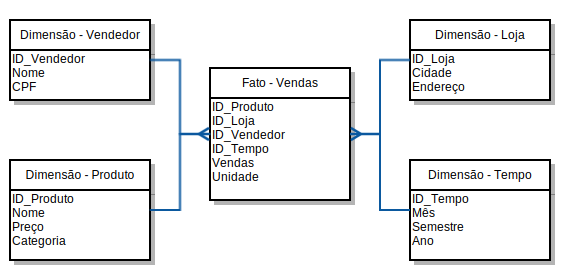
\includegraphics[width=13cm]{images/ex_olap.png}
	\caption{Representação de um modelo dimensional em um banco de dados relacional do tipo estrela.}
	\label{fig:exOlap}
\end{figure}

Os dados armazenados em um cubo OLAP passam por algoritmos de indexação, técnicas de armazenamento e outras otimizações que fazem com que as consultas realizadas nesta estrutura de dados, mesmo sendo complexas, tenham um alto desempenho no tempo de resposta para o usuário.

Um dos processo que fazem parte da modelagem de dados OLAP é o de extração, transformação e carga (do inglês ETL - \emph{Extract, Transform and Load}). Este processo consiste na extração de dados de fontes externas e na transformação dos mesmos, para que possam atender às necessidades de negócio. Posteriormente, estes dados são carregados em um \emph{Data Warehouse} ou em outros ambientes de banco de dados.

O processo de ETL é considerado o mais complexo e que consome mais tempo durante a criação de um ambiente de \emph{Data Warehouse/Business Intelligence}, pois consiste em movimentar e transformar os dados que irão servir como base para futuras decisões gerenciais. Portanto, os dados precisam estar precisos e consistentes. 
Muitas vezes as informações estão armazenadas em diferentes fontes de dados e não possuem um padrão de estrutural de dados \cite{KIM13}. Nestes casos, as etapas de extração e transformação precisam de um esforço para que os dados sejam tratados de forma homogênea.
























% ----------------------------------------------------------
% Ferramentas de Desenvolvimento
% ----------------------------------------------------------
\chapter{Ferramentas de Desenvolvimento}

\section{Linguagem Python}
A escolha de uma linguagem de programação foi uma peça-chave para possibilitar o desenvolvimento de scripts para preparação dos dados utilizados neste trabalho. Uma simulação de docagem molecular gera um grande volume de dados, e para tratá-los, foi necessário a utilização de uma linguagem que suportasse a manipulação desta massa de dados através de uma forma simples de desenvolvimento.

Python é uma linguagem na qual possui uma curva de aprendizado relativamente simples se comparada com as outras linguagens utilizadas no mercado atualmente. Esta característica é explicada pelo fato desta linguagem possuir uma estrutura de dados mais alto nível e uma abordagem simples, mas efetiva para programação orientada à objeto. Por possuir uma sintaxe clara e de tipagem dinâmica, se torna simples a legibilidade do código fonte \cite{pyt00}. 

A linguagem possui eficientes estruturas de dados de alto nível, como: listas, dicionário, data/hora e outros. Dessa forma, o desenvolvedor não se envolve com detalhes de baixo nível tais como manipulação de ponteiros, alocação de memória, etc. A biblioteca nativa do Python possui uma vasta coleção de módulos prontos para uso, inclusive para processamento de texto e expressões regulares. Também existe a possibilidade de adicionar \emph{frameworks} desenvolvidos por terceiros.

Outra característica importante desta linguagem é ser multiplataforma. Portanto, é possível a execução em ambientes Windows, Mac e todas as distribuições Linux. Esta característica possibilita que programas escritos nesta linguagem sejam portáveis para qualquer outra plataforma com facilidade \cite{pyt01}.

Pelo que se pode observar através de pesquisas, a linguagem Python está sendo amplamente empregada na área de bioinformática para auxiliar atividades de manipulação de dados, análise de arquivos e interações com banco de dados. Dessa maneira, observando as características citadas, o Python apresenta-se como uma linguagem ideal para ser empregada neste trabalho.

\section{Microsoft SQL Server Analysis Services}
O Microsoft SQL Server Analysis Services, ou SSAS como é conhecido, é uma ferramenta \emph{desktop} de \emph{Business Intelligence} desenvolvida pela empresa Microsoft que permite trabalhar com modelos multidimensionais OLAP e mineração de dados. O Analysis Services funciona como uma camada independente para visualização dos dados armazenados em um banco de dados, seja ele SQL Server ou não. A partir desta ferramenta é possivel criar modelagens multidimensionais, realizar consultas e relatórios, através de uma interface totalmente uniforme \cite{MIC13}.

Assim como outras ferramentas OLAP existentes no mercado, o Analysis Services é utilizado nas organizações principalmente para apoiar o processo de tomada de decisão. Como o modelo OLAP permite acessar a analisar os dados com uma grande flexibilidade, as empresas viram nestas características uma plataforma perfeita para integração e consolidação de informações de processos de negócio.

Por se tratar de uma ferramenta da Microsoft, as ferramentas do Microsoft Office possuem suporte para integração com o Analysis Services. Esta integração permite que ferramentas do pacote Office se tornem um fron-end para acesso aos dados corporativos e recursos de \emph{Business Intelligence}. Para as organizações esta integração se torna um benefício direto, pois a interface das ferramentas do pacote Office é conhecida pela maioria de seus usuários, não sendo necessário o investimento para treinamentos específicos.

Qualquer tipo de dado que esteja armazenado em um banco do Analisys Services pode ser importado para o Microsoft Excel através de uma conexão ativa. Este procedimento simplifica expressivamente a análise dos dados, realização de consultas \emph{on-line}, geração de relatórios, etc. O processo de setup e implantação do Analysis Services não requer conhecimentos avançados, e a sua utilização em conjunto com o Microsoft SQL Server apresenta uma curva de aprendizado rápida.

Para o desenvolvimento deste trabalho foi utilizado o Analisys Services em conjunto com o banco de dados Microsoft SQL Server. Um aspecto que contribuiu para utilização destas ferramentas foi a parceria existente entre a PUCRS e a Microsoft. O programa Microsoft DreamSpark permite aos alunos o uso destas e outras ferramentas sem que seja necessário a aquisição de licenças de uso.


\chapter{Materiais utilizados}
	
\section{Banco de simulações de docagem}

\section{Receptor Investigado}

\section{Ligantes Considerados}

\section{Script para preparação dos dados}

Com objetivo de automatizar o processo de preparação dos dados de simulações de docagem molecular, foi criado um script utilizando a linguagem Python. Este script é responsável pela sumarização dos dados resultante da simulação para posteriormente alimentar o modelo OLAP com os dados já organizados.

Através de uma fórmula matemática, faz-se um filtro para obtenção das ligações mais estáveis, enquanto as ligações que apresentam valores ruins, consideradas instáveis, são descartadas.

Os dados de entrada são carregados através de dois arquivos delimitados por vírgula (comma-separated values), onde cada um deles deve conter os resultados da simulação de docagem com as coordenadas do LIGANTE (?). Após a execução do script, tem-se como resultado os dados sumarizados e organizados, prontos para alimentar o modelo OLAP.

O procedimento executado por este script consiste nas seguintes etapas:

\begin{enumerate}
    \item bla
    \item bla
    \item bla
\end{enumerate}

mostrar cálculo  que é realizado para obter apenas os melhores resultados.
mostrar tabela de exemplo do resultado de saída do script.
\chapter{Desenvolvimento do modelo OLAP}

descrever como foi feito o levantamento dos residuos mais interesantes. Explicar que a lista dos mais presentes foi comparada com uma lista originalmente desenvolvida por um especialista de dominio. Encontrou se casos que estavam e nao estavam na lista, os que nao apareciam na lista constituem de residuos que se ficam ˜proximos”ao sitio de ligação, mas que na realidade estão fora do sítio.

descrever como  adicionar novas dimensoes baseadas em novos residuos

\section{Identificação de métricas}

\section{Identificação dos resíduos relevantes}
Um dos pontos mais importantes para responder aos questionamentos dos especialistas de domínio e fundamental para composição das dimensões, era saber quais eram os resíduos mais relevantes. A enzima InhA possui 268 resíduos \cite{KARANADUNOSM09} e o processo de identificação dos mais importantes leva em consideração o número de contatos do resíduo com o ligante. Na base de informações que foi resultado do processo de simulação de docagem, cada resíduo é representado por uma tripla contendo a sua localização espacial nos eixos x, y e z.

De acordo com o especialista de domínio, para ser considerado contato do resíduo com o ligante é preciso estar em uma distância entre 2 e 4 angstrom. Valores inferiores a 2 angstrom são descartados por serem considerados uma sobreposição. Desta forma é utilizado o cálculo da distância euclidiana entre os átomos do resíduo e do ligante \cite{KARANADUNOSM09} para encontrar estes valores, desprezando os átomos de hidrogênio conforme determinação dos especialistas de domínio. Quanto maior o número de contatos do resíduo com o ligante, mais relevante para o especialista é o resíduo. As regras para elencar os resíduos mais relevantes podem ser sumarizadas da seguinte forma:

\begin{enumerate}
    \item Distância de 2 a 4 angstrom são considerados contatos.
    \item Distância inferior a 2 angstrom são desconsideradas. 
    \item Descarte do cálculo para os átomos de hidrogênio.
    \item Quanto mais contatos, mais relevante.
\end{enumerate} 

Com base nestas prerrogativas foram selecionados os 10 principais resíduos mais relevantes para responder às questões dos especialistas conforme mostrado.

\begin{itemize}
	PHE_148 (Phenylalanine)
	ILE_193 (Isoleucine)
	GLY_95 (Glycine)
	THR_195 (Threonine)
	ILE_94 (Isoleucine)
	MET_198 (Methionine)
	MET_160 (Methionine)
	SER_19 (Serine)
	ILE_15 (Isoleucine)
	TYR_157 (Tyrosine)
\end{itemize}

\section{Dimensões}
	mostrar hierarquias de dimensoes
	
\section{Construção do modelo no Analisys Services}
	exibir a tabela pivotante com os valores medios (feb,rmsd)

\chapter{Resultados Obtidos}
	respostas às questões levantadas com os especialistas de domínio. entrevistas com o especialista, identificação das necessidades.
\chapter{Conclusão}

A modelagem OLAP para analisar experimentos de simulação de docagem molecular se mostrou eficiente conforme visto no capítulo \ref{cap:ResultadosObtidos}. Embora o conjunto de dados utilizado tenha sido relativamente pequeno, com 3100 conformações para cada um dos dois ligantes, o modelo OLAP construído deve funcionar conforme esperado para \emph{data sets} ainda maiores. Os processos de extração, transformação e carga dos dados utilizando a linguagem de programação Python foram bem sucedidos conforme visto no capítulo \ref{cap:DesenvolvimentoDoModeloOLAP}, e podem ser reutilizados em outros projetos de docagem sem necessidade de grandes alterações. 

A abordagem de utilização do modelo OLAP para análise de experimentos de docagem molecular não parece ser usual entretanto, com a sua eficácia comprovada, a tendência é que isto possa ser utilizado mais massivamente para cruzar os dados da simulação de forma bastante flexível, situação que hoje ainda limita os especialistas.


%----------------------------------------------------------------
% Aqui vai a bibliografia. Existem dois estilos de citação: use
% 'ppgcc-alpha' para citações do tipo [Abc+] ou [XYZ] (em ordem
% alfabética na bibliografia), e 'ppgcc-num' para citações
% numéricas do tipo [1], [20], etc., em ordem de referência.
%----------------------------------------------------------------
\bibliographystyle{ppgcc-alpha}
%\bibliographystyle{ppgcc-num}
\bibliography{tcc-bib}

%----------------------------------------------------------------
% Após \appendix, se iniciam os capítulos de Apêndice, com
% numeração alfabética.
%----------------------------------------------------------------
%\appendix
%\chapter{Meu primeiro apêndice}
%\chapter{My second appendix}

%----------------------------------------------------------------
% Aqui vão os "capítulos" de anexos. Cada anexo deve
% ser considerado um capítulo.
%----------------------------------------------------------------
%\anexos
%\chapter{Meu primeiro anexo}
%\chapter{My second attachment}

% E aqui (para a felicidade de todos) termina o documento.
\end{document}
